\lecture{Segurança em redes sem fio}{wireless}

\lecturetitle{\course}{\insertlecture}

\frame{\maketitle}

\begin{frame}{Referências}
  
  \begin{itemize}
  \item James F. Kurose; Keith W. Ross. Redes de computadores e a
    Internet: uma abordagem top-down. Addison-Wesley, 5a edição,
    2010.
  \item \href{http://www.windowsecurity.com/}{WindowsSecurity.com}
  \end{itemize}
\end{frame}

\begin{frame}{}
  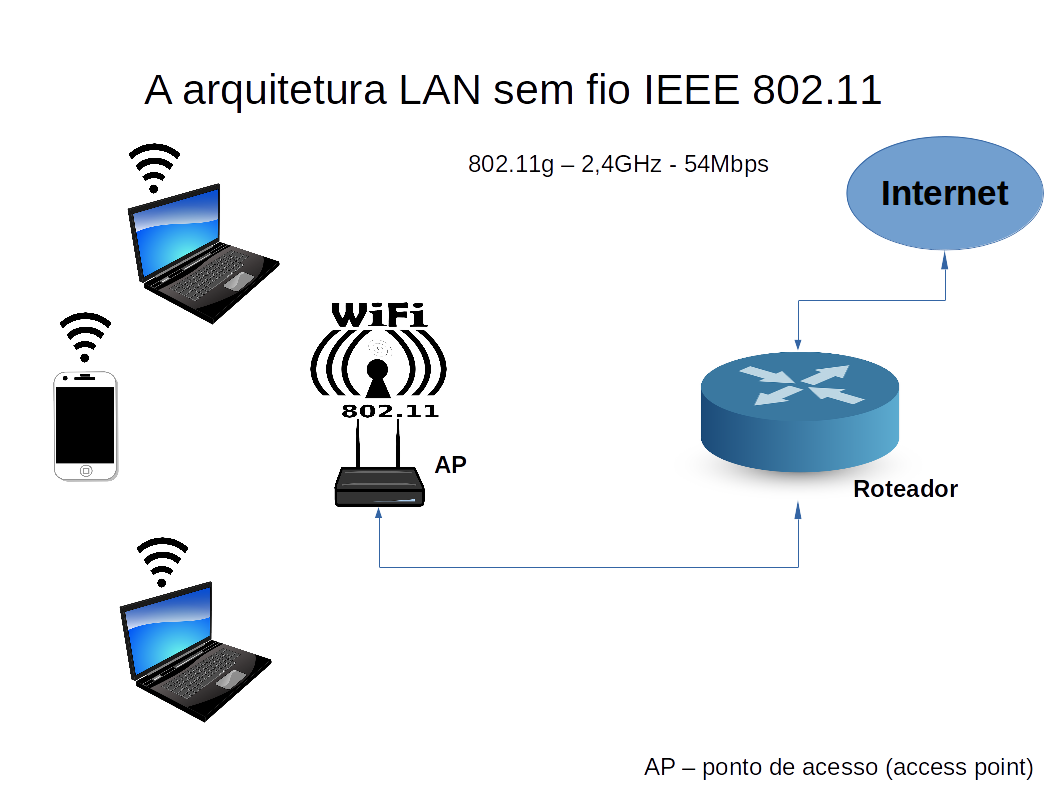
\includegraphics[scale=.39]{wifi.png}
  {\scriptsize 802.11n --	5Ghz -- 900Mbps}
\end{frame}

\section{\insertlecture}

\begin{frame}{Ataques comuns a redes sem fio}
  \large

  \begin{enumerate}[<+->]\setbeamercovered{transparent}
  \item Passivo
  \item Ativo
  \item {\em Man-in-the-middle}
  \item Congestionamento ({\em jamming})
  \end{enumerate}
  
\end{frame}

\subsection{Ataque Passivo}

\begin{frame}{Ataque Passivo}{Descrição}

  \begin{itemize}[<+->]\setbeamercovered{transparent}
  \item Ocorre quando alguém fica bisbilhotando o tráfego na rede.
  \item O bisbilhoteiro captura os pacotes da rede usando uma placa de
    rede no modo promíscuo e ferramentas como o
    \href{https://www.microsoft.com/en-us/download/details.aspx?id=4865}{\tt
      MS Network Monitor} (Windows) e
    \href{http://www.tcpdump.org}{\tt tcpdump} (Unix) ou
    \href{https://sourceforge.net/projects/airsnort/}{\tt AirSnort}.
  \item Ataques passivos em redes wireless são muito comuns.
  \end{itemize}
  
\end{frame}

\begin{frame}{Ataque Passivo}{Defesa}
  
  \begin{itemize}[<+->]\setbeamercovered{transparent}
  \item A única defesa contra a escuta passiva é criptografar o
    transporte na rede usando WEP ({\em Wired Equivalent Privacy}), VPN
    (rede virtual privativa), {\tt ssh} (secure shell), {\tt scp}
    (secure copy) sempre que possível.
  \end{itemize}
\end{frame}

\subsection{Ataque Ativo}

\begin{frame}{Ataque Ativo}{Descrição}
  
  \begin{itemize}[<+->]\setbeamercovered{transparent}
  \item Uma vez que o atacante colheu informações suficientes sobre a
    rede, os ataques ativos são parecidos com aqueles da rede com fio:
    \begin{itemize}
    \item Acesso não autorizado;
    \item Queda de serviço (DoS ({\em Denial of Service}), DDoS ({\em
        Distributed Denial of Service}));
    \item Roubo e interceptação de dados;
    \item Propagação de {\em malware};
    \item Envio de {\em spam}.
    \end{itemize}
  \end{itemize}
  
\end{frame}

\begin{frame}{Ataque Ativo}{Defesa}

  \begin{itemize}[<+->]\setbeamercovered{transparent}
  \item Filtro de endereço MAC (media access control);
  \item Uso de autenticação através de servidor RADIUS, com uso de
    firewall no servidor de autenticação.
  \end{itemize}
  
\end{frame}

\subsection{{\em Man in the Middle}}

\begin{frame}{\em Man in the Middle}
  
  \begin{itemize}[<+->]\setbeamercovered{transparent}
  \item Colocação de um ponto de acesso (AP) com o mesmo SSID (Service
    Set Identifier) de um AP existente na rede, com o objetivo de
    fazer com que os usuários tentem autenticar em um AP não
    autorizado.
  \item {\bf Defesa:} difícil de detectar exigindo monitoramento
    lógico e físico da rede.
  \end{itemize}
\end{frame}

\subsection{Ataque de Congestionamento}

\begin{frame}{Ataque de Congestionamento}

  \begin{itemize}[<+->]\setbeamercovered{transparent}
  \item Tipo especial de queda de serviço (DoS), específico para redes
    wireless, onde o atacante transmite ondas de frequência RF
    espúrias para interferir no sinal da rede.
  \item {\bf Defesa:} não é um ataque comum devido ao custo do
    equipamento para realizá-lo.
  \end{itemize}
  
\end{frame}

\begin{frame}{Segurança em Redes Wireless}
  
  \begin{itemize}[<+->]\setbeamercovered{transparent}
  \item Utilizar protocolos de criptografia: WEP ({\em Wired
      Equivalent Privacy}), WPA ({\em Wi-Fi Protected Access}), WPA2
  \item Dê segurança ao SSID:
\begin{itemize}[<+->]\setbeamercovered{transparent}
  \item Mude o SSID padrão;
  \item Mude o SSID em intervalos frequentes;
  \item Certifique-se de que o sistema não esteja aberto;
  \item Não use SSID fáceis e identificáveis;
  \item Mude a senha em intervalos frequentes, procurando não repeti-las;
  \item Use filtro de MAC;
  \item Use autenticação e IPSec (IP Security) se necessário.
\end{itemize}
\end{itemize}

\end{frame}


\begin{frame}{Ferramentas de Auditoria}
\href{https://www.aircrack-ng.org/}{Aircrack-ng}\bigskip

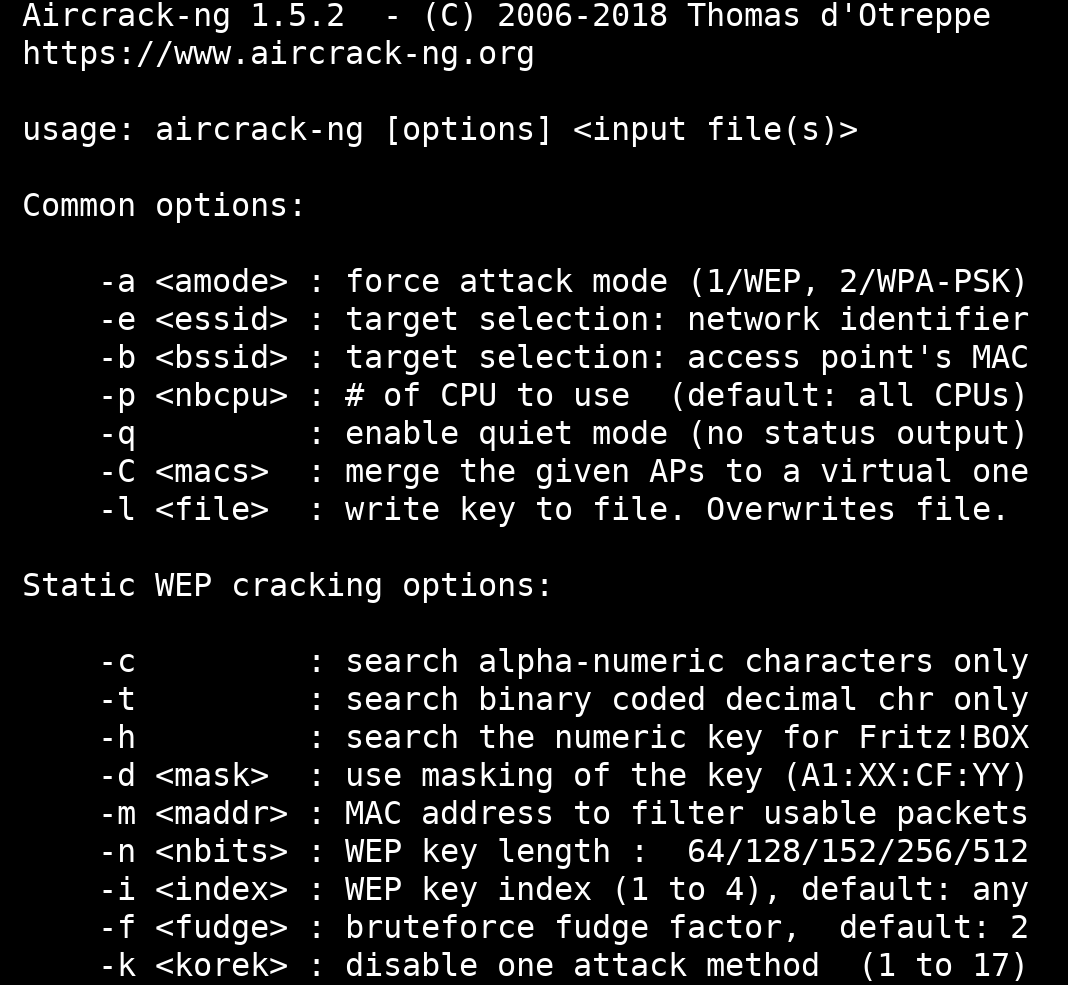
\includegraphics[scale=.2]{aircrack-ng.png}

\end{frame}

\begin{frame}{Ferramentas de Auditoria}
\href{https://play.google.com/store/apps/details?id=com.farproc.wifi.analyzer&hl=pt_BR&gl=US}{WiFi Analyzer} 
para Android\bigskip

 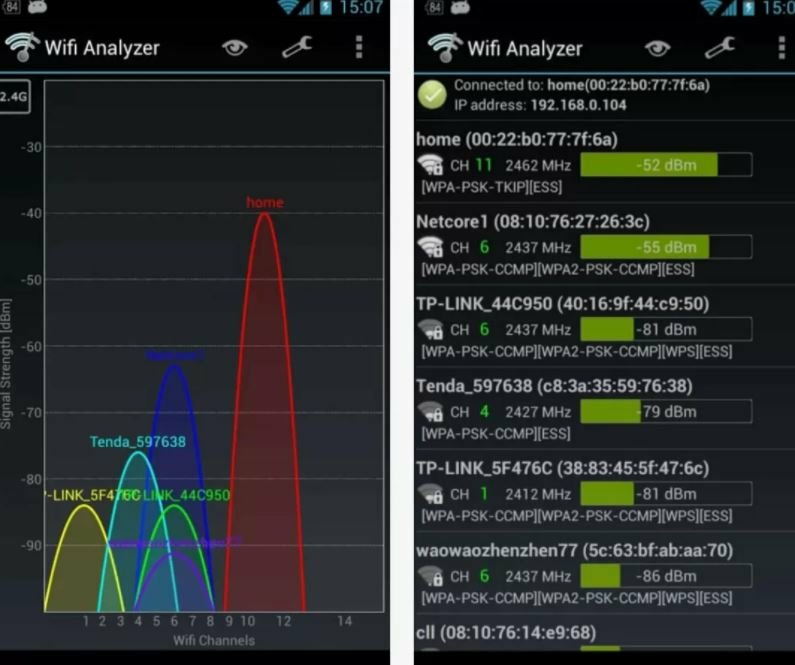
\includegraphics[scale=.275]{wifi-analyzer.png}
\end{frame}

\begin{frame}{Ferramentas}{Mais algumas}

\begin{itemize}
\item \href{https://www.kismetwireless.net/}{Kismet}
\item \href{https://github.com/savio-code/fern-wifi-cracker}{Fern Wi-fi Cracker}
\item \href{https://github.com/wiire-a/pixiewps}{PixieWPS}
\item \href{https://github.com/derv82/wifite2}{Wifite}
\item \href{https://www.wireshark.org/}{WireShark}
\end{itemize}

\end{frame}